\documentclass[border=6pt]{standalone}
% Shared preamble of every figure (included by each fig*.tex)
\usepackage{fontspec}
\setmainfont{DejaVu Sans}
\setmonofont{DejaVu Sans Mono}
\usepackage{amsmath,amssymb}
\usepackage{tikz}
\usetikzlibrary{positioning,arrows.meta,fit,calc,decorations.pathreplacing,shapes.geometric,backgrounds}
\definecolor{cdata}{HTML}{4C78A8}
\definecolor{cmodel}{HTML}{F58518}
\definecolor{chead}{HTML}{54A24B}
\definecolor{cgold}{HTML}{E45756}
\definecolor{cgrey}{HTML}{9D9D9D}
\definecolor{cfull}{HTML}{B279A2}
\tikzset{
  box/.style={draw, rounded corners=2pt, align=center, inner sep=4pt, font=\small, minimum height=8mm},
  data/.style={box, fill=cdata!15, draw=cdata!80!black},
  model/.style={box, fill=cmodel!18, draw=cmodel!80!black},
  head/.style={box, fill=chead!18, draw=chead!70!black},
  note/.style={font=\footnotesize, align=center, text=black!70},
  arr/.style={-{Stealth[length=2.2mm]}, thick, black!70},
}

\newcommand{\st}[1]{{\scriptsize\bfseries\color{black!55}#1}\\}
\begin{document}
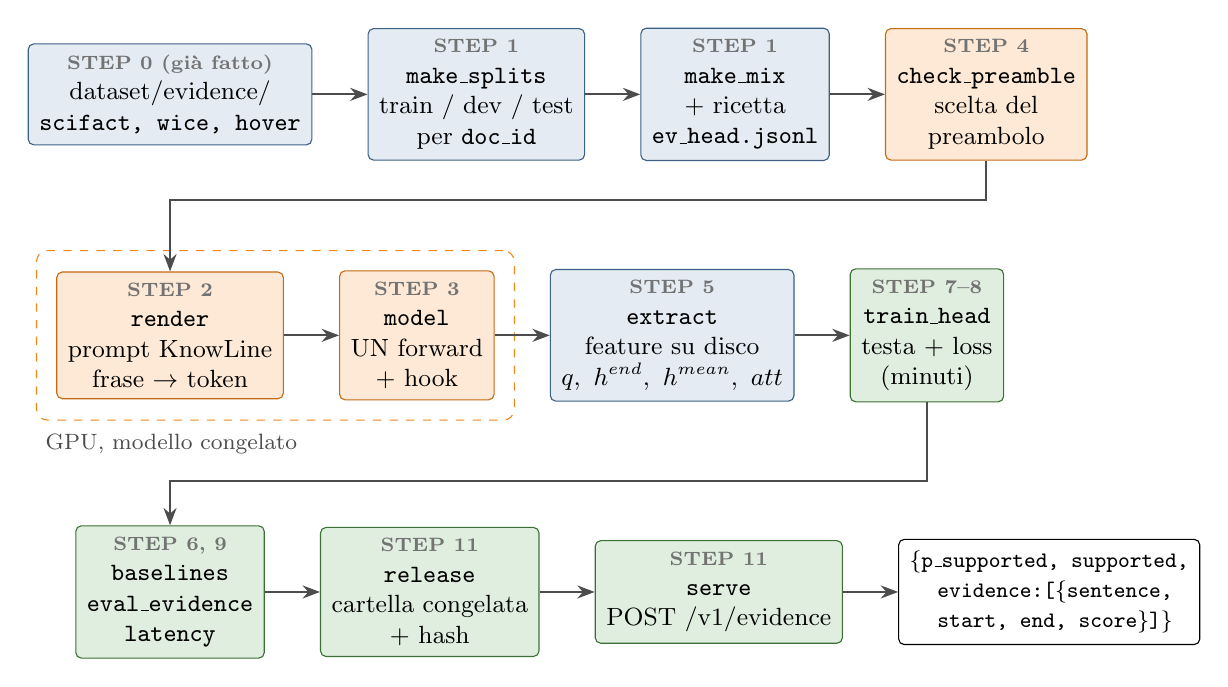
\begin{tikzpicture}[node distance=6mm and 7mm]
\node[data] (src) {\st{STEP 0 (già fatto)}dataset/evidence/\\\texttt{scifact, wice, hover}};
\node[data, right=of src] (split) {\st{STEP 1}\texttt{make\_splits}\\train / dev / test\\per \texttt{doc\_id}};
\node[data, right=of split] (mix) {\st{STEP 1}\texttt{make\_mix}\\+ ricetta\\\texttt{ev\_head.jsonl}};
\node[model, right=of mix] (pre) {\st{STEP 4}\texttt{check\_preamble}\\scelta del\\preambolo};
\node[model, below=16mm of src] (render) {\st{STEP 2}\texttt{render}\\prompt KnowLine\\frase $\to$ token};
\node[model, right=of render] (fwd) {\st{STEP 3}\texttt{model}\\UN forward\\+ hook};
\node[data, right=of fwd] (feat) {\st{STEP 5}\texttt{extract}\\feature su disco\\$q,\ h^{end},\ h^{mean},\ att$};
\node[head, right=of feat] (train) {\st{STEP 7--8}\texttt{train\_head}\\testa + loss\\(minuti)};
\node[head, below=16mm of render] (eval) {\st{STEP 6, 9}\texttt{baselines}\\\texttt{eval\_evidence}\\\texttt{latency}};
\node[head, right=of eval] (rel) {\st{STEP 11}\texttt{release}\\cartella congelata\\+ hash};
\node[head, right=of rel] (serve) {\st{STEP 11}\texttt{serve}\\POST /v1/evidence};
\node[box, right=of serve, fill=white] (out) {\footnotesize\texttt{\{p\_supported, supported,}\\\footnotesize\texttt{ evidence:[\{sentence,}\\\footnotesize\texttt{ start, end, score\}]\}}};
\draw[arr] (src) -- (split); \draw[arr] (split) -- (mix); \draw[arr] (mix) -- (pre);
\draw[arr] (pre.south) -- ++(0,-5mm) -| (render.north);
\draw[arr] (render) -- (fwd); \draw[arr] (fwd) -- (feat); \draw[arr] (feat) -- (train);
\draw[arr] (train.south) -- ++(0,-10mm) -| (eval.north);
\draw[arr] (eval) -- (rel); \draw[arr] (rel) -- (serve); \draw[arr] (serve) -- (out);
\begin{scope}[on background layer]
\node[fit=(render)(fwd), draw=cmodel, dashed, rounded corners, inner sep=2.5mm] (g) {};
\end{scope}
\node[note, anchor=north west] at ($(g.south west)+(0,-0.5mm)$) {GPU, modello congelato};
\end{tikzpicture}
\end{document}
